In the following we will outline out design of \thename{} and give a detailed
description of each area of functionality. The design is heavily tied to the
\thename{} specification, but further includes some considerations for
implementation, i.e.~the design of the implementation.

As previously mentioned, the primary aim of \thename{} is to provide an abstract
machine that is capable of supporting most of the modern programming paradigms
in an efficient manner. The overarching idea is that by exposing much of the
underlying low-level constructs we provide very flexible means for compilers to
do things the way that is most suitable for their particular requirements,
without having to conform to a tight object-model or strict type system. This
involves exposing constructs like virtual tables (see Section~\ref{NEEDED}) and
thread management (see Section~\ref{NEEDED}). Further the type system is aimed
at being strict enough to guarantee type safety but flexible enough for dynamic
languages. Compilers are free to select which features to utilize, meaning for
instance that for a strictly statically typed language, the dynamic typing
mechanisms can be disregarded and all method dispatches can be wired statically.
% TODO more?

\textbf{Note:} Because the specification is such a central document to the
design we will not cite the specification directly throughout the
thesis. Instead we refer to Appendix~\ref{appendix:spec} where the full
specification is included.

\subsection{Memory Model}
% TODO garbage collector
\thename{} uses the common stack and heap memory model. Stacks are local to
threads, and cross-thread references between stack elements are illegal. The
heap is a globally shared memory region in which values reside until they are
deallocated or cleaned by the garbage collector. Threads store and retrieve
values on the heap using the same addresses, thus facilitating shared
data. Machine type values such as \code{Int8} and \code{Boolean}
(Section~\ref{NEEDED} details the available types and type system) typically
reside on the stack but can be boxed (see Section~\ref{NEEDED}) and placed on
the heap.

\subsection{Execution Model}
%TODO: tasks and transactions
The model of execution defines how, where and by whom code is executed during
run-time. All code in \thename{} is executed in the context of a thread (see
Section\ref{sec:design:threading}), and all threads are spawned from an original
``main'' thread in which execution begins. This allows language implementations
to use multi-threading features of \thename{}, but also to ignore them and run
everyting in a single thread without having to worry about creating and
destroying threads.

\subsection{Object Model}
%TODO: more
The object model defines how heap objects are layed out in memory and how their
content is described by the type system. The object model used \thename{} is
heavily based on the C++ Itanium ABI\cite{itanium}. That means that all heap
objects include a pointer to a virtual table which is essentially a statically
created lookup table that maps integer indices to pieces of code
(i.e.~sub-routine addresses). Further, and different from the Itanium ABI, the
virtual tables contain type information about the heap
object. Figure~\ref{fig:design:heap-object-layout} shows how a heap object is
stored in memory. The bootstrapped virtual table is created by the machine and
can be thought of as the fundamental ``Object'' type that all other objects
inherit from.

\begin{figure}[H]
  \centering
  \begin{tikzpicture}
  \draw (9, -1) node (b_vtbl) {
    \begin{tabular}{c}
      Bootstrapped\\vtable
    \end{tabular}
  };

  \drawstruct{(5,0)}
  \structcell[freecell]{Virtual table} \coordinate (vtbl_e) at (currentcell.east); \coordinate (vtbl_w) at (currentcell.west);
  \structcell[freecell]{Type information}
  \structcell[freecell]{Lookup table}
  \structname{Virtual table}

  \drawstruct{(5,-5)}
  \structcell[freecell]{KV1} \coordinate (hm) at (currentcell.west);
  \structcell[freecell]{KV2}
  \structname{Hash map}

  \drawstruct{(0,0)}
  \structcell[freecell]{Virtual table} \coordinate (ho_vtbl) at (currentcell.east);
  \structcell[freecell]{Hash map} \coordinate (ho_hm) at (currentcell.east);
  \structcell[padding]{Object data}
  \structname{Heap object}

  \draw[->, thick] (ho_vtbl) -- (vtbl_w);
  \draw[->, thick] (ho_hm) -- (hm);
  \draw[->, thick] (vtbl_e) -- (b_vtbl);
\end{tikzpicture}
  \caption{Heap object memory layout}
  \label{fig:design:heap-object-layout}
\end{figure}

\subsection{Executable File Format}
%TODO: more
\thename{} reads executable files written in the Executable Linkable Format
(ELF). ELF is a very popular format for executable binary files that is used in
most Unix based systems (OpenBSD, Linux, Solaris, etc\cite{NEEDED}). That alone
enables much easier porting of existing libraries and frameworks to
\thename{}.


\subsection{Types}
%TODO: more
Types are represented differently in the ELF files and internally in the
machine. DWARF\cite{dwarf} is used in the executables.

The internal type system is described in Section~\ref{sec:implementation:types}.


\subsection{Stack Management}
%% Basic
%% Stack vs. Register
%%% (see background)
%% Threaded
%% Stack element
%%% Type
%% Manipulation (instr)

Stack is an abstract data type, fundamental in the fields of algorithms and
computer science. It is a very simple model only requiring two essential
functions, {\it push} and {\it pop}, as visualized in
figure~\ref{fig:stack}. Push adds an element to a stack of elements, while pop
removes the top most element. As an analogy, imagine a pile of dishes. When
adding a new dish it becomes the new top-most dish in the stack. This sequence
of adding and taking from a collection of element is called Last In, First Out
(LIFO).
\begin{figure}[h]
  \centering
  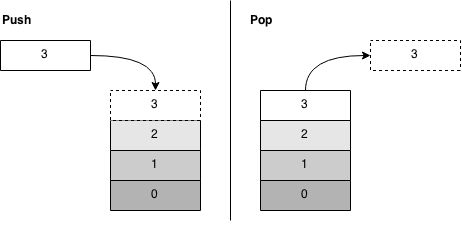
\includegraphics[scale=0.6]{images/stack.png}
  \caption{Stack push and pop operations}
  \label{fig:stack}
\end{figure}

% The stack was first introduced in 1946 by Alan Turing, while he was working on
% the Automatic Computing Engine (ACE)~\footnote{Automatic Computing Engine (ACE):
% \url{http://en.wikipedia.org/wiki/Automatic_Computing_Engine}} at the National
% Physical Laboratory (NPL)~\footnote{National Physical Laboratory:
% \url{http://en.wikipedia.org/wiki/National_Physical_Laboratory_(United_Kingdom)}}
% in the UK:
% \begin{quote}
%   [Alan Turing] outlined a method for leaving one line of work being carried out
%   on the computer, calling up a subsidiary line, and then returing to the first
%   line when finished with the subsidiary line. He called the calling up and
%   returning routines BURY and UNBURY.~(\textcite[82]{newton})
% \end{quote}
% Here, BURY and UNBURY are synonymous with push and pop.

% @book{newton,
% author    = "David E. Newton",
% year      = 2003,
% title     = "Alan Turing : a study in light and shadow",
% publisher = "[Philadelphia]: Xlibris",
% ISBN      = 9781401090791
% }

Although, essentially, one cannot take the second element from top without first
removing the top most element, the model can easily be modified to support such
operations. For instance, a common stack operation is {\it peek}, which reads
the value of the top element without actually removing it. This can easily be
done by popping, storing the value and pushing it back to the stack. Other
operations can be implemented in a similar fashion.

\subsubsection{Stack vs. Register Machine}
Machines can implement the stack model virtually and execute it directly in
hardware, but as we are designing an abstract machine, we will only discuss the
virtual aspect. Regardless, such a machine is commonly called a \term{stack
  machine}.

The most common notation in arithmetic formulas and statements are the infix
notation, where the operator is written between its operands: $1 + 2$. One can
express the same statement with prefix notation, also called \term{Polish
  notation}: $+\ 1\ 2$. When programming stack machines, one uses what is called
the \term{reverse Polish notation}, which is in fact postfix notation:
$1\ 2\ +$. By using this notation, one can easily convert this into stack
operations, where $1\ 2\ +$ becomes:
\begin{stackops}
  \op{push 1}{1}
  \op{push 2}{2,\ 1}
  \op{add}{3}
\end{stackops}

Here the {\tt add} operation pops two elements, adds them together and pushes
the result back onto the stack.

As briefly discussed in the~\ref{sec:background} section, a register machine
TODO

\subsubsection{Stack Organization}
% All stacks will initially have a single activation frame

The stacks will not be limited in size, as the stacks can be implemented as heap
object which can grow dynamically. Through out this report, we will say that the
stacks \term{grows downwards}. This is because physically, the top most element
of the stack is located at a low address in the host computers
memory. Therefore, as more elements are pushed to the stack, they will get
higher addresses, making the stack grow downwards in memory.

A stack element will consist of some type information and a reference to its
content, or data. The type information will include its declared type, but also
an actual type. For statically typed languages, these will most likely (TODO: ?)
be the same. For dynamic languages this is required to hold track of an
element's type, as its allowed to assign a value type an element, which was
originally declared with an other type.

\subsubsection{Stack Manipulation}
As mentioned above, there will we instructions for doing simple stack
manipulations, for instance {\tt push} and {\tt pop}. As we will see later,
these two instructions alone will be very limiting, and make the job of writing
a compiler very tedious. Therefor, we will need more instructions, making more
complex manipulations more convenient.

When we later describe the execution model of the machine, we will see that we
need instructions for pushing an popping elements further up the stack. For
instance, if we want to access the arguments given to a subroutine, they will be
located up the stack. The compiler will therefor need an effective method of
duplicating that element onto the top of the stack, making is accessible for
further computation. Also it will need to push an element to a specific position
up the stack, effectively returning a value to the caller.

Such versions of the push and pop operations will take an displacement argument,
saying how many places up the stack it is to push to or pop from. To make this
as convenient as possible, the displacement will be from the top of the stack,
meaning displacement 0 will be the top of the stack. Exception handling will
have to be utilized when using a displacement which is not allowed, for instance
outside the stack or its own scope.

Lets call these two instructions {\tt pushElement} and {\tt
  storeElement}. Unlike {\tt push}, which adds a new element to the stack, the
specification defines {\tt pushElement} to overwrite the element at the given
displacement. This is more convenient as this does not change the displacement
of the following elements, though it requires some planning, as there will have
to be an element on the stack with the purpose of being overwritten. {\tt
  storeElement} will pop of the top-most element and place it at the given
displacement.

Also, unlike our previous stack example, the {\tt push} instruction, or rather
the {\tt pushElement} instruction, will not take a value as an argument. Rather
it will take the element at the given displacement and push onto the top of the
stack. There will be separate instructions for adding new elements onto the
stack, for instance {\tt pushConstant}.

Here we can see some simple operations using the {\tt pushElement} and {\tt
  popElement} operations.
\begin{stackops}
  \op{-}{3,\ 1,\ 1}
  \op{pushElement 0}{3,\ 1,\ 1,\ 3}
\end{stackops}


\subsection{Threading}
\label{sec:design:threading}
Big chip manufacturers like Intel, have always been under big pressure to
deliver ever faster processors, year after year. For around the last decade, the
technological development of processors has been focused adding cores rather
than increasing the clock speed, which already started to stagnate around
2004~\cite{sutter}. With multiple processors, or popularly called a multi-core
processor, processes may actually run in parallel, i.e. running at the same
time, rather than just concurrently where multiple processes actually share the
same processor.

A thread is typically the smallest unit of executable instructions by a
processor. A process being run by an operating system therefore had one thread
which the operating systems scheduler delegated CPU time to. With multi-core
processors, the notion of a single process having multiple threads arose, making

Although multi-threading is a very interesting feature, it also raises a lot of
challenges when designing machines. Different threads cannot directly read and
write to the same place, or address, in memory without taking data races into
account, which is a common mistake when writing multi-threaded programs. If
multiple threads are reading and writing to the same memory, it is impossible
for the threads to base any logic on it, as another thread can change its value
at any time, effectively pulling the rug from under you. This problem as been
named the mutual exclusion problem, and is solved by using synchronization
structures.

Our machine will both support threading and synchronization structures
therefor. As we are using a stack machine, each thread has to have its own
state, including its own stack. In other words, all stacks are private and
cannot be shared across threads. This can though be facilitated by using heap
object which are referenced from multiple threads' stack.

\subsubsection{Tasks and Transactions}
TODO
% Multiple executables may execute simultaneously.
% Task and transaction semantics is supported. A transaction is considered
% executed by the thread starting it. A spawned task is independent of the spawn-
% ing thread and may be executed by the spawning thread or some other thread.
% However, tasks will not migrate between threads so the thread which started
% execution of a task will also complete the task.

% Tasks do not share stacks with the spawning thread, spawning task, or any
% other task. Implementations may, however, execute tasks using the stack of the
% executing thread. The executed task is not allowed to access any stack space
% beyond its initial set of stack elements. The implementation must throw an
% exception if any such offending access is attempted.

\subsubsection{Thread Pool}
Creating and destroying system threads is not free. If a new thread is created
on demand, it would create significant overhead. Another problem with this model
is the risk of resource thrashing. If there is no limit on the number of threads
that can be created, it can intentionally or unintentionally be exposed to heavy
abuse. A solution to both of these challenges is having what is called a
\term{thread pool}. On machine initialization, a set number of threads is
pre-initialized and stored in a data structure. When a thread tries to spawn a
new thread, it is given one from the thread pool. If the thread pool is empty,
it has to wait for a thread to become vacant.

This model, although effective, also brings with it some
challenges. Specifically, when the thread pool is empty. The spawning thread
cannot stop and wait until a new thread is vacant, as this would block the whole
thread. Rather, the machine will use a work queue. A work queue manages the
thread pool so other threads does not need to wait for a thread to become
vacant, and thereafter fight with each other of whom gets to take it. The
spawning threads would give the task which it wants run in a new thread, to the
work queue. The queue would monitor the thread pool and as soon as a thread
becomes free, it would take the task first in the work queue and run in.

\subsubsection{Errors and Exceptions}
Two types of errors can occur; internal errors in the machine and errors
produced by the program the machine is executing. Internal errors will most
likely occur in some child thread and not in the process' original thread. If
that is the case we would stop that thread and gracefully stop the machine if it
cannot safely continue. If the error occurs in the process' original thread, we
will in most cases still be able to catch the signal sent by the OS and
gracefully stop.

When the program being executed produces an \term{exception} it will percolate
up through a defined set of exception handlers until it is handled. If there is
no way of handling the exception it called an uncaught exception. It that case
the machine will print some information on the exception and stop. It will not
attempt to join all threads (TODO) as it cannot know how long this will
take. Therefore all threads are exited and memory is freed, ensuring no memory
leaks.

TODO: Exception handling


\subsection{Types}
The machine will have a built-in set of types. These are broken into simple
types, arrays, reference types, composite types and meta types. These will
effectively lay the foundation for arbitrary new types new to be mapped upon.

The simple types are will consist of:
\begin{description}
\item[Integer] Will include all combinations of 8-bit, 16-bit and 32-bit, signed
  or unsigned, integer numbers. E.g. {\tt Int32} and {\tt UInt16}.
\item[Boolean] A {\tt Boolean} type with the values `true` or `false`.
\item[Float] 32-bit or 64-bit floating point numbers, in the IEEE 753-1985 or
  IEEE 755-1985 standard representation, respectively named {\tt Ieee32} and
  {\tt Ieee64}.
\item[Address] Unsigned integer value representing a memory address, named {\tt
    Address}. This is considered unsafe, and will therefore only be possible in
  code declared as `unsafe`.
\item[Abstract] Type which can take any value at run-time, named {\tt
    AnyType}. Large values will be boxed on the heap to make space for it.
\end{description}

We will also lay the foundation for composite types, making them easy to define
through recursion. They will simply reference those of the simple types to
compose new composite types.

% reference

The machine will have a set of reference types, with the most fundamental being
the {\tt Reference <t>} type. This allows heap objects to be referenced from the
stack. As the name infers, it will take a type of the object it referenced as
argument. In the opposite scenario, there is a {\tt StackReference <t>} type,
allowing passing references directly to stack references. This type may not be
boxed, nor passed to threaded tasks. This will save programs from major pitfalls
in concurrent programs (?).

To support variable argument calling conventions, letting a subroutine take an
arbitrary number of arguments, a special reference type is needed. This is done
through an {\tt ArgumentReference}, allowing a subroutine to iterate over its
given arguments. Also, to referencing a subroutine will be done through a {\tt
  CodeReference <signature>}, taking the signature which it implements. This is
a meta type, described below.

% arrays

The machine will support two types of arrays; a static and a dynamic
type. Both will be generic, taking the type of its values. This could be to
other arrays, allowing an array to be multi-dimensional. The static variant will
also take a lower and higher limit of values, aptly named {\tt StaticArray
  <t><lowerLimit><higherLimit>}. The dynamic variant will not take the limits,
as therefore named {\tt DynamicArray <t>}. To allow it to grow dynamically, it
will be instanced and put on the heap. It will therefore be referenced through a
{\tt Reference} type.

% composite

To support custom types, similar to a struct in the C programming language,
there will be a {\tt Composite <t+>} type. This will take an arbitrary number of
type arguments, describing its member. Though not visible from the type
signature, each member will have a name, allowing for convenient referencing (TODO).

Lastly, the machine will have a set of meta types, describing types by them
selves. These include {\tt Type}, {\tt Signature} and {\tt TypeSignature}. (TODO)


% Examples of how to map things to our model ()
%% Classes
%% Inheritance
%% HoF
%% Polymorphism

% Type system
%% Representation (DWARF)
%% Typed instructions
%% Run-time type checking
%% Dynamic types
%%% !!!

% Executable format
%% ELF
%%% It's tried-and-true
%%% Everybody else uses it so we can port stuff easier

% Object model
%% Virtual tables
%% Hash maps
%%% How is it different from using vtables
%%% The efficiency of them
%% Dynamic dispatches

% Threading
%% Tasks and transactions
%%% Shared stack elements
%% ?!
%% Thread Pool
%%% Resource thrashin

% Closures

% Memory management
%% Garbage collection

% ISA
%% Highlight the most important instructions, explain how they facilitate the above


% Mem model
%% Standard heap and stack, stack per thread, global heap
%%

%%% Local Variables:
%%% mode: latex
%%% TeX-master: "../report"
%%% End:
